\begin{center}
Le plan est muni d'un repère orthogonal.
\end{center}

\subsubsection*{Partie A}
On considère la fonction $P$ définie sur l'intervalle $[-5~;~3]$ par :
\[P(x) = 2x^2 + x - 10.\]

\begin{enumerate}
\item 
	\begin{enumerate}
	\item Déterminer les racines de $P$.
	\item En déduire l'axe de symétrie de la parabole d'équation $y = P(x)$.
\end{enumerate}

\item Établir le tableau de signe de la fonction $P$ sur l'intervalle $[-5~;~3]$.
\end{enumerate}

\subsubsection*{Partie B}
On considère la fonction $f$ définie et dérivable sur l'intervalle $[-5~;~3]$ dont on donne ci-dessous la courbe représentative $C_f$.

\begin{center}
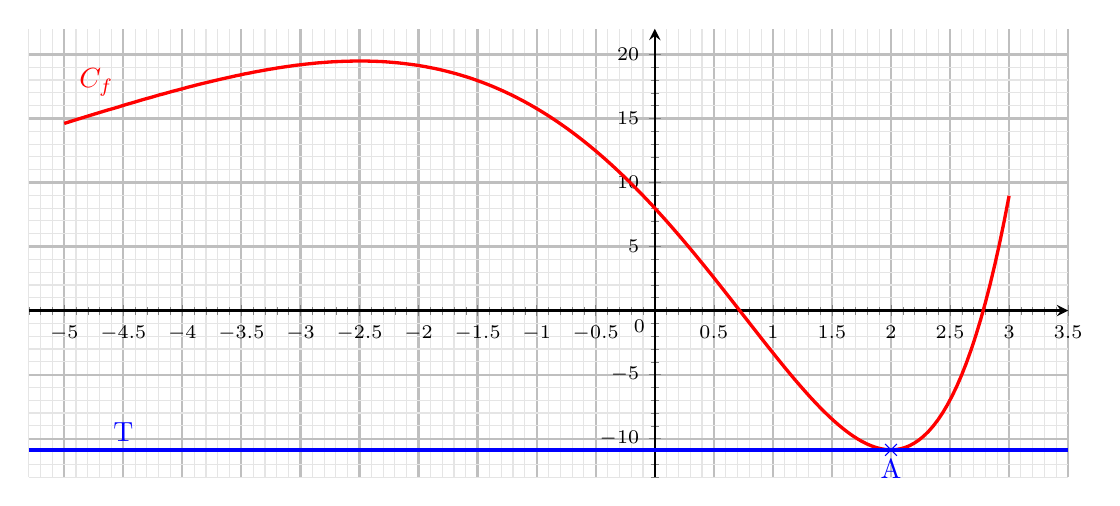
\begin{tikzpicture}
\begin{axis}[
    xmin=-5.3, xmax=3.5,
    ymin=-13, ymax=22,
    samples=200,
    domain=-5:3,
    axis lines=middle,
    axis line style={thick},
    xtick distance=0.5,
    ytick distance=5,
    tick label style={font=\scriptsize},
    x tick label style={
        /pgf/number format/.cd,
        fixed,
        fixed zerofill,
        precision=1,
        /tikz/.cd,
        /pgf/number format/zerofill=false
    },
    xticklabel={
        \pgfmathprintnumber{\tick}
    },
    x=1.5cm,
    grid=both,
    major grid style={gray!50, thick},
    minor grid style={gray!20, thin},
    minor x tick num=4,
    minor y tick num=4,
]
\addplot[red, very thick, restrict y to domain=-13:22] {(4*x^2 - 14*x + 8)*exp(0.5*x)};
\node[font=\scriptsize, below left] at (axis cs:0,0) {0};
\node[above left, color=red] at (axis cs:-4.5,16) {$C_f$};
\addplot[blue, mark=x, mark size=3pt] coordinates {(2,{(4*2^2 - 14*2 + 8)*exp(0.5*2)})};
\node[blue, below] at (axis cs:2,{(4*2^2 - 14*2 + 8)*exp(0.5*2)}) {A};
\pgfmathsetmacro{\yA}{(4*2^2 - 14*2 + 8)*exp(0.5*2)}
\addplot[blue, very thick] coordinates {(-5.3, \yA) (3.5, \yA)};
\node[blue, above] at (axis cs:-4.5,-11) {T};
\end{axis}
\end{tikzpicture}
\end{center}

La tangente $T$ à la courbe $C_f$ au point A d'abscisse 2 est horizontale.

\begin{enumerate}
\item Donner la valeur du nombre dérivé $f'(2)$.

\item Résoudre, avec la précision permise par le graphique, l'inéquation $f'(x) < 0$.

\item On sait que la fonction $f$ a pour expression sur l'intervalle $[-5~;~3]$ :
\[f(x) = (4x^2 - 14x + 8)\e^{0,5x}.\]

Démontrer que, pour tout $x$ appartenant à l'intervalle $[-5~;~3]$, on a :
\[f'(x) = P(x)\e^{0,5x}.\]

\item En utilisant les résultats de la \textbf{partie A}, dresser le tableau de variation de la fonction $f$ sur l'intervalle $[-5~;~3]$. \textit{(Il n'est pas demandé de calculer les images)}.
\end{enumerate}

